%!TEX root = ../thesis_a4.tex

\chapter{Literature review}
\label{sec:SOA}

\section{Introduction}

The literature review presented in this chapter is divided into two parts.
Firstly, we summarise existing work on the definition and characterisation of tagging systems.
We describe what a tagging system is, how different authors have proposed to categorize tagging systems, the motivations that users have when annotating content and the different types of tags resulting from these annotations. Additionally, we discuss problems that are typically found in tagging systems and highlight some of the solutions that are commonly proposed. 
Secondly, we focus on existing specific literature about tag recommendation systems.
We outline the different approaches that have been proposed for tag recommendation, describe how these approaches are normally evaluated, and finally summarise research about the impact that tag recommendation is expected to have on the folksonomies of tagging systems.


\section{Tagging systems}
\label{sec:SOA:tagging_systems}

Tagging systems systems have been well studied since the popularisation of tags in online sharing platforms and the social web in general.
From a broad perspective, tagging is the process of assigning tags to content resources.
Considering that this can be done manually by users or automatically by machines, tagging approaches can be divided into \emph{manual} and \emph{automatic} tagging~\citep{Wang2012}.
The focus of this thesis is on manual tagging systems.
Manual tagging systems can provide different levels of assistance during the tagging process (e.g.,~the system can suggest popular tags to the user) or provide no assistance at all, but in both cases users have the final decision on whether or not to assign a given tag to a content resource. Fig.~\ref{fig:manual_tagging_interfaces} shows the manual tagging interface of three online multimedia sharing sites.
Contrastingly, automatic tagging systems are designed to automatically add tags to resources without the need (or very little need) of human intervention. 
%Typically, these systems analyse content resources to extract low-level features, and then machine learning algorithms are trained on the basis of these features to be able to predict tags that are suitable for the resources being annotated. 
%Another common pattern for automatic tagging is the definition of a multidimensional feature space (based on the aforementioned low-level features) in which similarity measures can be defined to select content resources similar to a given target. If the similar resources have already been annotated with some tags, then these tags can be propagated to the target resource. These automatic approaches are known as model-based, and search-based automatic tagging respectively~\citep{Wang2012}. %Maybe find some references of these systems in \citep{Wang2012} section 2.2
Even though in this thesis we will not deal with automatic tagging systems, these are closely related to the tag recommendation systems that will be discussed later in this chapter, and thus we give an overview of them in Sec.~\ref{sec:soa:tag_recommendation}.


\begin{figure}[t]
  \centering
  \subbottom[]{
    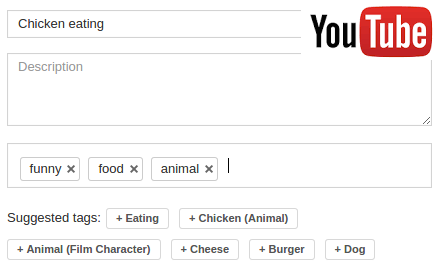
\includegraphics[width=6cm]{ch02_soa/pics/ss_youtube}}
  \hspace{0.5cm}
  \subbottom[]{
    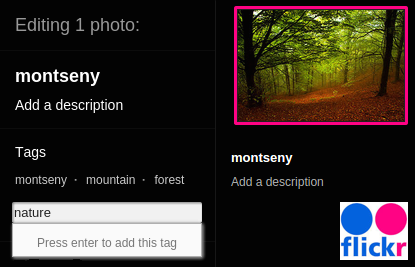
\includegraphics[width=5.65cm]{ch02_soa/pics/ss_flickr}}
  \subbottom[]{
    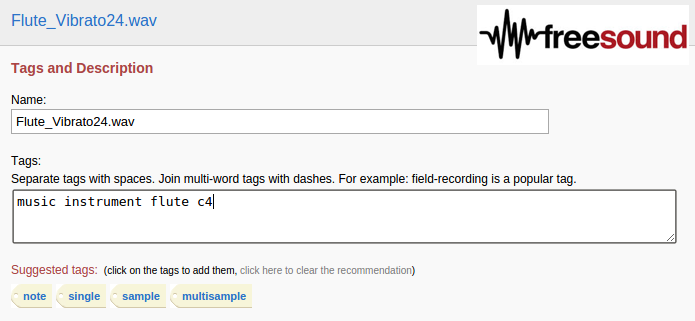
\includegraphics[width=9.47cm]{ch02_soa/pics/ss_freesound}}
  \caption[Examples of manual tagging system interfaces]{Examples of manual tagging system interfaces for (a) YouTube, (b) Flickr, and (c) Freesound. In this examples, both YouTube and Freesound annotation interfaces provide a number of suggested tags, whereas the Flickr interface does not.}
  \label{fig:manual_tagging_interfaces}
\end{figure}


In tagging systems, the individual tags that are assigned to a content resource typically represent annotations about different information dimensions or facets which, when considering the whole tagline, conform a description of the resource.
%For example, a tagline for a sound representing a recording of street ambience in Barcelona might include the following tags: \{\atag{barcelona}, \atag{street}, \atag{car}, \atag{h4n}, \atag{noisy}\}.
For example, a tagline for a sound representing a recording of the ambience in ``La Boqueria'' market in Barcelona, might include the following tags: \{\atag{coins}, \atag{barcelona}, \atag{boqueria}, \atag{atmosphere}, \atag{market}, \atag{noise}, \atag{people}\}\footnote{This example is actually taken from a sound shared in Freesound. It can be accessed in the following URL: \url{http://www.freesound.org/people/helenacm/sounds/101792/}.}.
%In that case, \atag{barcelona} indicates a specific location, \atag{street} conveys information about the generic place where the recording takes place, \atag{car} enumerats an object appearing in the recording, \atag{h4n} indicates the recording device that has been used, and \atag{noisy} describes an accoustic property of the recording.
In this case, the tags \atag{barcelona} and \atag{boqueria} indicate a specific location of the recording, \atag{market} conveys information about a generic place, \atag{people} and \atag{coins} list sound-producing elements appearing in the recording, \atag{noise} describes an acoustic property of the recording, and \atag{atmosphere} provides a possible generic classification of the type of audio. Other tags could be added, for example, to indicate the recording device used to capture the audio, or the specific time when the recording was made.
These tags are not introduced with a formal structure, and users can not indicate explicit relations among them.
The tags in the tagline, and by extension the aggregate of all distinct tags that form the folksonomy of a tagging system, are organised in a flat namespace, meaning that there is no explicit nor predefined hierarchy in which tags can be projected. 
Hence, the tagging activity is considered a categorisation process rather than a classification process, where the different tags convey information about possibly overlapping facets without formal structure~\citep{Jacob2004,halpin2006}. Conversely, formal classification systems organise items in unambiguous and exclusive concept hierarchies (or taxonomies) with a predefined and controlled vocabulary~\citep{golder2006}. %Threfore, tagging systems and their resulting folksonomies are often compared with formal classification systems and controlled vocabularies~\citep{golder2006}.
It has been argued that the use of tags instead of taxonomies with controlled vocabularies to annotate resources has two main advantages.
On the one hand, tags can better adapt to the annotation requirements of resources which might not be contemplated in controlled vocabularies. This brings a lot of flexibility as users can intuitively introduce previously non-existing tags to annotate unexpected content properties~\citep{Mathes2004,shirky2005ontology,Quintarelli2005,halpin2006,Sen,Fichter2006,Wu2006,Macgregor2004}.
On the other hand, when using tagging systems, users do not need to learn and understand the specific terms and organisation of a taxonomy, reducing the cognitive load of the annotation process and smoothing its learning curve~\citep{Quintarelli2005,shirky2005ontology,Fichter2006}. This is one of the reasons why tagging systems have become widespread in the social web and online sharing platforms in particular~\citep{Cattuto2006}.
%\citep{Cattuto2006}: ``It has been argued that the surging popularity of collaborative tagging is due to its comparatively small cognitive overhead with respect to taxonomic categorization''
However, tagging systems do exhibit significant disadvantages when compared with formal classification systems (see Sec.~\ref{soa:tagging_problems}). 


 
%%% Categorization of Tagging systems
\subsection{Types of tagging systems}
 
\cite{marlow2006} propose a categorisation for tagging systems according to seven dimensions, and discuss the implications of design choices that can be made for each dimension.
In Table~\ref{tab:tagging_systems_in_dimensions} we show some of the most popular online sharing platforms categorised according to their tagging system's characteristics and the dimensions proposed by~\cite{marlow2006}.   
The first dimension, ``tagging rights'', indicates which users of the tagging system can assign tags to resources. In some systems, only the owner of a resource can assign tags to it, while in other systems resources can be tagged by any user.
As we have seen in the introductory chapter, such a design choice leads to the emergence of either a narrow or broad folksonomy, respectively.
The second categorisation dimension, ``tagging support'', divides tagging systems according to the level of assistance given to the user during the tagging process. 
On the one hand, there are blind systems in which users are given no particular support during the tagging process. On the other hand, there are systems that feature mechanisms with different levels of complexity to suggest tags to users or guide the annotation process. Authors suggest that non-blind tagging systems reinforce the convergence of the vocabulary in the folksonomy (see Sec.~\ref{sec:soa:impact_tag_recommendation}).
The third categorisation dimension, ``aggregation model'', specifies whether the tags assigned by different users to a single resource are considered as a set of unique tags or as a union of all tags (bag of tags).
Hence, this dimension is only applicable to those tagging systems where resources can be tagged by multiple users (broad folksonomies). The different aggregation models constrain the available tagging statistics for each resource.
The fourth dimension proposed by~\cite{marlow2006} is the ``object type'', and defines the nature of the resources being tagged (e.g.,~web pages, bibliographic material, audio, video, images, etc.). The authors suggest that the type of resource has numerous implications on the resulting tags and folksonomy, hypothesising that resources without a direct textual representation (e.g.,~multimedia resources) require different kinds of annotations.
The fifth dimension, ``source of material'', separates tagging systems in those which the content to be tagged is supplied by users of the platform (typically user generated content or content from external sources like web pages), or by the platform itself. Authors suggest that the incentives that users have for tagging the content will be different depending on the source of the material.
Finally, the sixth and seventh dimensions are ``resource connectivity'' and ``social connectivity'', and indicate whether the resources or users of the system are explicitly organised in groups based on similarity, shared interests or any other aspects. \cite{marlow2006} suggest that explicit social or resource connectivity can contribute to the emergence of localised folksonomies for the defined groups, yielding particular tagging behaviours which are distinguishable from the global behaviour.
\cite{Sen} also proposed a categorisation of tagging systems that is very similar to the above described.
Although it only consists of four dimensions (``tag scope'', ``item ownership'', ``tag selection'' and ``tag sharing''), almost direct equivalences can be drawn.
%Besides Marlow's categorisation, a similar categorisation scheme for tagging systems is proposed by~\cite{Sen} which is based in four dimensions. These dimensions are very close to those proposed by~\cite{marlow2006}, and rough equivalences can be drawn: the ``tagging rights'' dimension proposed by ~\cite{marlow2006} corresponds to~\cite{Sen} ``tag scope'',  ``source of material'' by ~\cite{marlow2006} corresponds to~\cite{Sen} ``item ownership'', and finally a combination of ``tagging support'' and ``aggregation model'' dimensions find the equivalence in the ``tag selection'' and ``tag sharing'' dimensions proposed by~\cite{Sen}.
%In this thesis we mainly work with data gathered from Freesound. When analysing Freesound's tagging system characteristics with the dimensions proposed by~\cite{marlow2006} in mind, we see that Freesound features a narrow folksonomy (only the owner of a resource can annotate it) in which user-generated audio recordings are annotated. There is no explicit social connectivity among users of Freesound, but resource connectivity is sometimes present as audio recordings can be grouped into ``packs''
%Also, it worth mentioning that during the development of this thesis, a tag recommendation system was introduced in Freesound, thus altering the tagging support. 
%Furthermore, the source and type of material annotated in Freesound are user-generated audio recordings, and there is no explicit social connectivity among users of Freesound but resource connectivity is sometimes present as audio recordings can be grouped into ``packs''.
%In Table~\ref{tab:tagging_systems_in_dimensions} we show some of the most popular online sharing platforms categorised according to their tagging system's characteristics and the dimensions proposed by~\cite{marlow2006}. 
%In this thesis we mainly work with data gathered from the tagging system of Freesound. As it can be observed, Freesound features a narrow folksonomy (only the owner of a resource can annotate it) in which user-generated audio recordings are annotated. There is no explicit social connectivity among users of Freesound, but resource connectivity is sometimes present as audio recordings can be grouped into ``packs''. Furthermore, it is worth mentioning that during the development of this thesis, a tag recommendation system was introduced in Freesound. For more details on Freesound's characteristics, see Appendix~\hyperref[appendix:Freesound]{A}.


\begin{table}
\begin{threeparttable}
\centering
\ra{1.3}
\tiny
\begin{tabular}{@{}P{1.5cm}P{1.1cm}P{1.1cm}P{1.2cm}P{1.2cm}P{1.2cm}P{1.2cm}P{1.2cm}@{}}%
\toprule
%
\includegraphics[width=10cm]{ch00/pics/table_todo}
 & Flickr & YouTube & Soundcloud & Freesound & Delicious & Bibsonomy & CiteULike \\
 \midrule
\textbf{Tagging rights} & Owner & Owner & Owner & Owner & Everyone & Everyone & Everyone \\
\textbf{Tagging support} & Blind & Tag rec. & Auto-completion & Tag rec. & Tag rec. & Tag rec. & Blind \\
\textbf{Object type} & Photos & Video & Music and sounds & Sounds & Bookmarks & Biblio. ref., bookmarks & Biblio. ref. \\
\textbf{Source of material} & User-generated & User-generated & User-generated & User-generated & User-provided & User-provided, user-generated & User-provided, user-generated \\
\textbf{Resource connectivity} & Albums & Categories & Sets & Packs & - & - & - \\
\textbf{Social connectivity} & Groups, Followers & Channels, Followers & Groups, Followers & Followers & Followers & Groups & Groups, Followers \\
\bottomrule
\end{tabular}

\caption[Popular online sharing sites categorised in the dimensions defined in~\cite{marlow2006}]{Popular online sharing sites categorised in the dimensions defined in~\cite{marlow2006}. As the functionalities of some of these systems changed over time, we list here its characteristics in their state at the time of this writing. Note that the ``aggregation model'' dimension is not included in the table because it is typically not available.} 
\label{tab:tagging_systems_in_dimensions}
\end{threeparttable}
\end{table}



%%% User motivations for tagging 
\subsection{User motivations for tagging}
\label{soa:user_motivations}

\begin{table}[p]
\begin{threeparttable}
\centering
\ra{1.2}
\footnotesize
\begin{tabular}{@{}lp{9cm}@{}} \toprule
\textbf{Name} & \textbf{Description}  \\ 
\midrule 

Future Retrieval & Tags that users add to facilitate the future retrieval of the annotated resources. These tags can describe particular properties of a resource which are relevant to a broad audience and can be effectively used for indexing purposes. However, future retrieval tags can also include information which is only relevant to the user performing the annotation such as a tag like \texttt{toread}, which is typically used as a future reminder for the annotator. \\

Contribution and Sharing & These are tags that serve the purpose of categorising resources into rather common concepts and facilitate in this way future retrieval for other users of the platform. \\

Attract Attention & Some users choose to add popular tags when annotating their own resources to deliberately increase their reachability. This particular case can have a negative impact in the quality of the annotations if popular tags are chosen that have no relation with the actual content. \\

Play and Competition & Some tagging systems feature interfaces in which the annotation process is presented as an entertaining activity where users can, for instance, cooperate on annotating a resource. These systems are typically known as ``games with a purpose''~\citep{Ahn2006}. The most well known example of a game with a purpose in the tagging field is the ESP game~\citep{VonAhn2004}, in which pairs of users need to concurrently annotate a particular resource and are rewarded a number of points in accordance with their agreement in the chosen tags. \\

Self Presentation & These are tags that bear some aspect of the identity of the user that annotates a resource.~\cite{marlow2006} show, as an example of this kind of tags, the tag \texttt{seen live}, which sets a personal relation between the annotator and the resource. \\

Opinion Expression & Tags that users add with the purpose of expressing their subjective judgement or opinion about a resource. \\

Task Organisation & Similarly to some tags that could be in the future retrieval category, task organisation tags are used for organising resources through associated tasks that a particular user relates with the resource (e.g.,~\texttt{todo}, \texttt{toread}). \\

Social Signalling & Tags can be chosen to convey contextual information about a resource. For example, the name of the event in which a photo has been taken. In this case, users might be motivated by communicating their presence at that event. \\

Money & In some cases, users are being paid to annotate resources, typically through the use of platforms like the Amazon Mechanical Turk (\url{http://www.mturk.com/mturk/welcome}). \\%)$^a$. \\%\footnote{\url{http://www.mturk.com/mturk/welcome}}. \\

Technological Ease & Users can be also motivated by the ease of use of tagging systems (and sharing platforms in general) to annotate resources, so that the easier the tagging process is, the more likely users will be to annotate resources. \\
\bottomrule
\end{tabular}
\caption[Potential tagging motivations listed by~\cite{Gupta2010}]{Potential tagging motivations listed by~\cite{Gupta2010}.}
\label{tab:tagging_motivations}
%\begin{tablenotes}
%    \item[a] \url{http://www.mturk.com/mturk/welcome}.
%\end{tablenotes}
\end{threeparttable}
\end{table}

Several authors have studied the motivations or incentives that users have when tagging online resources~\citep{Mathes2004,marlow2006,golder2006,Sen,Xu2006,Ames2007,Gupta2010}.
\cite{marlow2006} propose a high-level categorisation of potential user motivations in two categories: ``organisational'' and ``social''. 
The ``organisational'' category includes tagging activities motivated by the aim of bringing a particular structure and organisation to contributed resources. In this case, users might develop particular tagging patterns and also adopt common patterns observed in other users of the tagging system. Tags under the ``organisational'' category should, in general, ease the future retrieval of the resources being tagged.
Tagging activities under the ``social'' category include the listing of user opinions and other communicative aspects that allow users to express themselves.
Besides these two broad categories,~\cite{marlow2006} also describe several more specific potential motivations for tagging resources.~\cite{Gupta2010} summarise these more specific categories along with others found in the literature~\citep{Mathes2004,golder2006,Xu2006,Sen,Ames2007}, and finally enumerate ten specific and non-exclusive categories which exemplify possible user motivations for tagging resources. Table~\ref{tab:tagging_motivations} lists these categories and provides a brief explanation for each one.
%These different motivations are tightly coupled with different kinds of tags that result of the annotation process~\cite{marlow2006}. That point is discussed below on Sec.~\ref{soa:types_of_tags}.

Besides these categorisations, of particular interest is the work by~\cite{Ames2007}, in which an empirical tagging study is carried out with participants being interviewed about their motivations when tagging pictures to be uploaded to Flickr.
In this study, the authors classify the responses provided by the interviewed participants in similar categories as those listed in Table~\ref{tab:tagging_motivations}. The observed motivations are, basically, those related to expressing user's opinions or relation with the photos to other known users of the system such as family or friends (roughly corresponding to ``self presentation'', ``opinion expression'' and ``social signalling'' categories of Table~\ref{tab:tagging_motivations}). Moreover, motivations related to the organisation of the resources (for easing future retrieval to both the owners of the photos and to other users of the system) are also repeatedly reported. Of particular relevance is the fact that, according to the interviews, participants are not aware of all potential motivations and benefits of tagging systems when annotating resources, and the decisions of which tags to choose are taken in an intuitive way rather than in an informed fashion. In relation to this, in a study by~\cite{marlow2006}, also with Flickr tagging data, authors suggest that the more resources a user has tagged, the more aware the user is about the relevance of chosen tags and annotation quality. In other words, as users learn to tag, their motivations change.




\subsection{Types of tags}
\label{soa:types_of_tags}


\begin{sidewaystable}
\begin{threeparttable}
\centering
\ra{3.0}
\footnotesize
\begin{tabular}{P{2.2cm}:L{1.8cm}:L{1.8cm}:L{1.8cm}:L{1.8cm}:L{1.8cm}:L{2.2cm}:L{1.8cm}:L{1.8cm}}
\toprule
\multicolumn{9}{l}{} \\[-1.05cm]
\textbf{\cite{Sen}} & \multicolumn{5}{c:}{Factual\tnote{a}} & Subjective & \multicolumn{2}{c}{Personal\tnote{a}} \\ %\hline
\textbf{\cite{cantador2010}} & \multicolumn{3}{c:}{Content-based} & \multicolumn{2}{c:}{Context-based} & Subjective & \multicolumn{2}{c}{Organisational} \\ %\hline
\textbf{\cite{Xu2006}} & Content-based & \multicolumn{2}{c:}{Attribute} & \multicolumn{2}{c:}{Context-based} & Subjective & \multicolumn{2}{c}{Organisational} \\ %\hline
\textbf{\cite{golder2006}} & What or who it is about & What is & Who owns it & \multicolumn{2}{c:}{Refining other categories} & Identifying qualities or characteristics & Task organisation & Self reference \\ %\hline
\textbf{\cite{Bischoff2008}} & Topic & Type & Author or owner & Time & Location & Opinions and qualities & Usage context & Self reference \\ %\hline
\textbf{\cite{Gupta2010}} & Content-based & Attribute & Ownership & \multicolumn{2}{c:}{Context} & Qualities and characteristics & Or\-ga\-ni\-sa\-tio\-nal and Purpose & Self reference\\
\multicolumn{9}{l}{} \\[-0.85cm]

\bottomrule
\end{tabular}

\begin{tablenotes}
    \item[a] These categories are also listed in \cite{Gupta2010}.
\end{tablenotes}

\caption[Types of tags, adapted and extended from the works of~\cite{cantador2010} and~\cite{Bischoff2008}]{Types of tags according to the kind of information conveyed about resources. This table is adapted and extended from the works of~\cite{cantador2010} and~\cite{Bischoff2008}.}
\label{tab:tag_types}
\end{threeparttable}
\end{sidewaystable}

In the previous section we have seen how some authors categorise tags in terms of potential user motivations or incentives. 
Another dimension in which tags can be categorised is on the basis of the kind of information that these convey about resources.
In that direction, several authors have proposed different, but highly related categorisations which are summarised in Table~\ref{tab:tag_types} and which are generic enough to be applied in tagging systems of different domains~\citep{golder2006,Sen,Xu2006,Bischoff2008,Gupta2010,cantador2010}. 
Among these categorisations featuring broader tag categories (upper rows in Table~\ref{tab:tag_types}), we find particularly meaningful the four-class categorisation proposed by~\cite{cantador2010}. Tags under ``content-based'' category describe the objects and qualities of a resource (e.g.,~content-based tags might enumerate the musical instruments that are present in an audio resource or its music genre). Tags under ``context-based'' category provide information about the context in which the resource was created (e.g.,~the location where a photo was taken or the time of the year in which a video was recorded). ``Subjective'' tags are those which express personal opinions that the tagger has about a resource at hand, such as quality judgements or mood annotations. Finally, ``organisational'' tags annotate resources with information that is, a priori, only useful for the annotator of the resource such as reminders related to the resource or self-referencing comments.
As can be seen in Table~\ref{tab:tag_types}, the other proposed broad categorisations are very similar~\citep{Sen,Xu2006}. Contrastingly, categorisations proposed by~\cite{golder2006}, \cite{Bischoff2008}, and \cite{Gupta2010}, include more fine-grained categories that can be easily understood as subdivisions of those broader categories mentioned above. 

Empirical research on the categorisation of tags has also been performed. \cite{Simons2008} analyses the Flickr tagcloud and performs a manual classification of the tags into a list of categories crafted to fit the data. By mapping these tailored categories to the broader categories proposed by~\cite{cantador2010}, it can be seen that around 66\% of tags belong to either ``content-based'' or ``context-based'' categories. The remaining 33\% can be classified as ``subjective'' or ``organisational'' tags. 
Similarly,~\cite{Bischoff2008} perform an analysis on the distribution of tags among their proposed categories using data from Delicious, Last.fm and Flickr. After a manual classification of a sample of all used tags, 55\% of the tags belong to either ``topic'', ``type'' or ``location'' categories, which are related to the broader ``content-based'' and ``context-based'' categories defined by~\cite{cantador2010}.
Furthermore, \cite{cantador2010} propose a rule-based method for automatically classifying tags into their proposed four broad categories. The method is based on the use of natural language processing techniques and YAGO\footnote{\url{http://www.mpi-inf.mpg.de/departments/databases-and-information-systems/research/yago-naga/yago/}.}, an external knowledge base. By performing a part-of-speech analysis of the tags and matching them to concepts of the YAGO knowledge base, the authors are able to determine to which category a tag belongs. Using data collected from Flickr, the authors performed the classification and found that, among those tags whose category could be predicted, 64\% are considered to be either ``content-based'' or ``context-based'' tags, while the others belong to ``subjective'' or ``organisational'' categories. As can be observed, these results are consistent with those reported by~\cite{Simons2008} and~\cite{Bischoff2008}.

By comparing Tables~\ref{tab:tagging_motivations} and~\ref{tab:tag_types}, it can be easily seen that tag types and tagging motivations are tightly coupled.
We explained before in Sec.~\ref{tab:tagging_motivations} that~\cite{Ames2007} found that users are more motivated for introducing tags expressing subjective opinions and self-references than to introduce tags describing the nature of the resources for their organisation. Considering this observation, we would expect to find more tags corresponding to the ``subjective'' and ``organisational'' categories rather than to the ``content-based'' and ``context-based'' categories, which is not what has been observed by~\cite{Simons2008},~\cite{Bischoff2008}, and~\cite{cantador2010}.
Interestingly, among the resulting types of tags and motivations, not all of them are equally suitable for generating useful metadata for indexing the content of online sharing platforms. In the case of systems featuring narrow folksonomies such as Flickr or Freesound, those tags that convey information which is meaningful not only to the owners of a resource but also to the other users of the platform, are crucial in order to successfully index content. Thus, according to the categorisation proposed by~\cite{cantador2010}, the presence of ``content-based'' and ``context-based'' tags is more desirable than ``subjective'' and ``organisational'' tag types. Conversely, in broad folksonomies such as Declious or Last.fm, ``subjective'' and ``organisational'' tags can be as important as ``content-based'' and ``context-based''. This is because in these systems users mainly tag for their self-organisation, and the used tagging conventions do not necessarily need to be meaningful to other users of the platform~\citep{DeMeo2013}.


%%% Problems of tagging systems
\subsection{Tagging systems' problems and solutions}
\label{soa:tagging_problems}

We have seen that the flexibility provided by tagging systems typically carries a number of well known problems which limit the possibilities of indexing, searching and browsing in sharing platforms~\citep{golder2006,halpin2006,Guy2006}. A very common problem is the presence of tags with typographical errors and tags formed with several concatenated words.~\cite{Guy2006} found that 40\% of Flickr tags and 28\% of Delicious tags contain misspellings or compound words that could not be mapped into a dictionary. These tags become less relevant, as a tagging system most probably treats misspelled versions of words as different tags. Moreover, word concatenation easily leads to different variations of a single concept.
In addition to that, it is very common that a single tag might have several different meanings (polysemy), and thus some users might employ it thinking of one meaning and some other users might employ it thinking of another meaning. Without a successful method for disambiguation, this results in making relations between resources which are semantically not meaningful. For example, search results might display resources related to different meanings of the query terms. Conversely, it is also quite common that several tags refer to a single concept (synonymy) and users employ them indistinctly. In that case, some relevant resources might be left out of the results of a query because systems are not generally aware of synonymy relations. Polysemy and synonymy problems have been empirically evaluated by~\cite{Spiteri2006}, analysing data of folksonomies gathered from Delicious, Furl and Technorati\footnote{Furl is a no longer existing online sharing platform. In it, users shared web bookmarks (similarly to Delicious). Technorati is currently a publisher advertising platform, but used to be a blog tracking site (\url{http://www.technorati.com/}).}, where it was found that between 12\% and 22\% of the tags potentially feature these kind of problems.

Another common problem of tagging systems is the use of tags that are only relevant for a specific user or the use of tagging conventions which are only known by particular users. These kind of tags convey information which is not generally useful to the community, and therefore their organisational value is limited. For example, a user might annotate resources using very particular tags whose meaning is not known to other users, and these annotations might appear to be totally unrelated to the resources.~\cite{Kennedy2006a} found that, given a Flickr image, only 50\% of the tags can actually be easily related to the content of the image or even to the image at all.
That can particularly become a problem in tagging systems with narrow folksonomies, in which tags that have a shared meaning for the community should be reinforced to improve indexing, searching and browsing possibilities~\citep{Guy2006}. 
Furthermore, a typical problem of tagging systems is the \emph{lack of tags}. Some studies show that user provided tags tend to be incomplete. As an example,~\cite{Sigurbjornsson2008} show that 50\% of images in Flickr have less than four tags, and~\cite{Zhao2010} show that YouTtube videos have an average of five tags, which means that annotations are not very comprehensive.

On an even higher level, different tagging styles can also create a problem for the tagging system if there are no signs of consensus.
If a common vocabulary is not shared among users, the informational value of tags is lessened and resources become less reachable (see Sec.~\ref{sec:soa:impact_tag_recommendation}). Furthermore, the co-existence of different languages in a single tagging system can also become an obvious problem~\citep{halpin2006}.
Overall, most of these issues are inherent to the vocabulary problem~\citep{Furnas1987}, caused by the lack of well defined tagging guidelines and the different rationales that users can apply during the tagging process. Nevertheless, the design and functionalities of tagging systems potentially have a big influence on the tagging behaviour when annotating resources, and this could be shaped so that typical tagging problems can be lessened~\citep{Wang2012}.

% on another level: specificity of the tags in relation to the content (eg. an hour of video, where the tag applies?). (Relate cost of tagging with batch tagging functionality in Flickr (\citep{Wang2012}), an tagging quality with tagging of specific regions in images or subclips in videos (mention that idea applies to soundcloud sets) tagging studies (search references in \citep{Wang2012}, annotation B).)

% The Structure and Form of Folksonomy Tags: The Road to the Public Library Catalog
%\citep{Spiteri2006}: analyse a month of data from delicious, furl (bookmark sharing) and technorati (blog sharing) and compare the emerging folksonomy with National information Standards Organization (NISO) guidelines for constructing controlled vocabularies.
%- most of the tags $\approx$95\% are nouns instead of adjectives and adverbs, which fits NISO recommendations
%- problems arise with inconsistent use of plural forms and ambiguous tags (compared to NISO recommendations), and that could be improved during the annotation phase

In order to mitigate some of the above mentioned tagging systems' problems, many authors have focused on approaches in which manual tagging is combined with computer algorithms to try to ``optimise'' the taglines introduced by users. Some of these approaches are meant to be used at the time when users annotate newly uploaded resources, but others are focused on improving already existing annotations.
\cite{Wang2012} introduce the concept of \emph{assistive tagging} to refer to these approaches, and propose a classification into three groups. 
The first group, ``tagging with data selection and organisation'', includes these approaches in which tagging systems automatically detect already existing resources which are poorly described and ask users to annotate them. In this case, many users can contribute to improving the annotations of a pool of selected resources, and the system can prioritise which content should be annotated first~\citep{Huang2008,Wang2011a}. % and optimise, for example, the implicit creation of training sets for machine learning algorithms that can later be used to automatically annotate other unlabelled resources~\citep{Huang2008,Wang2011a}.
A similar idea consists of the organisation of data to be annotated in clusters, which then become the smallest unit of tagging. Tags assigned to particular clusters are propagated to all resources of that cluster. This approach has been mainly applied in photo tagging, with clusters formed on the basis of face recognition algorithms~\citep{Suh2004,Cui2007,Tian2007}, or on the basis of sub regions of an image~\citep{Tang2010}. In the latter case, it is interesting that by clustering photos according to smaller regions and then annotating the regions, the tags can be applied to many photos at once. 
These methods are oriented to batch tagging of resources which, in the context of an online sharing site, does not necessarily need to be performed at upload time by the authors of the content. Instead, it can be performed in a collaborative fashion by other users of the platform.

The second group of assistive tagging strategies, ``tag processing'', includes those approaches in which existing annotated resources are post-processed in order to automatically correct or refine the descriptions. For example, in photo tagging systems, images can be segmented and machine learning algorithms can be trained to learn the mapping of introduced tags with particular regions, and then propagate the tags to other images with similar regions~\citep{Liu2010b,Feng2010,Liu2011}. Similar ideas, applied at a temporal level rather than at the region level, have been applied to video tagging~\citep{Ulges2008}. Furthermore, systems can be trained to compute a relevance score for the tags assigned to a resource based on the analysis of its content, and filter in this way tags with low scores~\citep{Liu2009,Li2009,Chen2010a,Fan2010}.
Another approach for post-processing user provided annotations is the use of knowledge bases like WordNet~\citep{Miller1995} to extend annotations with synonyms and hypernyms or filter out tags which are unrelated according to the knowledge base~\citep{Liu2010a}. % approach with topic modeling \cite{Xu2009} and matrix decomposition \cite{Zhu2010a}
Finally, the third group of assistive tagging strategies identified by~\cite{Wang2012}, ``tag recommendation'', consists of approaches in which tagging systems suggest tags to users during the annotation process, thus potentially shaping users' tagging behaviour. These systems are the main topic of the present thesis, and are discussed in the following section.



%%% Tag recommendation

\section{Tag recommendation}
\label{sec:soa:tag_recommendation}

The existing literature on tag recommendation systems is generally focused on recommendation systems for image or social bookmarking sharing sites.
However, highly related to tag recommendation systems are automatic tagging systems.
In essence, automatic tagging systems and tag recommendation systems share their main goal: generating a set of relevant tags for a given resource.
Hence, a lot of the techniques described in the literature are applicable to the two kinds of systems.
In this section, we summarise a number of approaches that, either being more focused on tag recommendation or automatic tagging, are of relevance to contextualise the work described in this thesis. Nevertheless, we put our focus on the systems designed for the task of tag recommendation.

Tag recommendation systems can be classified according to the main source of information that is used in the recommendation process.
In general, approaches can be separated in \emph{i)} systems based on the content analysis of the resources, \emph{ii)} systems based on the folksonomy of a tagging system, and \emph{iii)} systems based on contextual data~\citep{Wang2012}. 
In the following sections, we review existing literature on each one of these approaches.
Table~\ref{tab:soa_methods_comparisson} shows a summary of all approaches reviewed in these sections.


\begin{sidewaystable}
\begin{threeparttable}
\centering
\ra{1.1} %0.2
\tiny
\begin{tabular}{@{}p{3.0cm}p{1.35cm}P{2.3cm}P{1.6cm}P{2.3cm}p{1.6cm}p{1.45cm}T{1.0cm}p{2.5cm}@{}}
% HEADER
\toprule
& \textbf{Focus} & \textbf{Type of resource} & \textbf{Type of approach} & \textbf{Based on} & \textbf{Sharing platform} & \textbf{Evaluation method} & \textbf{Dataset size} & \textbf{Evaluation} \hspace{0.5cm} \textbf{measures} \\
\midrule
% ROWS
\cite{Barnard2003} & Auto Tag. & Image & CO & IF, MOD & - & Prediction & 9,000 & Increase of $\precision$ \\
\cite{barrington2007} & Auto Tag. & Sound & CO & AF, MOD & - & Search & 1,305 & $\precision$, $\recall$, $\fmeasure$ \\
\cite{jaske2007} & Tag. rec. & Bookmarks, Music & FO & CF, FK, PE & Bibsonomy, Delicious, Last.fm & Prediction & 361 74,854 1,853 & $\precision$, $\recall$, $\fmeasure$ \\
\cite{Sood2007} & Tag. rec. & Blog posts & CT & TF, SIM & Technorati & User assess. Prediction & 225 & $\precision$, $\recall$, $\fmeasure$ \\
\cite{Anderson2008} & Tag. rec. & Image & FO, CO & CC, IF, MOD & Flickr & Prediction & 924 & $MRR$, $S$, $P$ \\
\cite{Chen2008a} & Tag. rec. & Image & CO & IF, MOD & Flickr & User assess. & 930 & \tnote{a} \\
\cite{Garg2008} & Tag. rec. & Image & FO & CC, PE & Flickr & Prediction & 50M & $MRR$, $S$, $P$ \\
\cite{Li2006} & Auto Tag. & Image & CO & IF, MOD & Flickr & User assess. Prediction & 5,411 47,000 & $\precision$, $\recall$, $\fmeasure$, $S$ \\
\cite{Lipczak2008} & Tag. rec. & Bookmarks & FO & CC, PE & Bibsonomy & Prediction & 274,139 & $\precision$, $\recall$, $\fmeasure$ \\
\cite{Naaman2008} & Tag. rec. & Image & CT & GPS & Flickr & Prototype & 100,000 & \tnote{b} \\
\cite{Sigurbjornsson2008} & Tag. rec. & Image & FO & CC & Flickr & User assess. & 331 & $MRR$, $S$, $P$ \\
\cite{Song2008} & Tag. rec. & Bookmarks & FO & CC, TCL & Bibsonomy & Prediction & 32,279 & $\precision$, $\recall$, $\fmeasure$ \\
\cite{turnbull2008} & Auto Tag. & Music & CO & AF, MOD & - & Prediction & 500 & $\precision$, $\recall$, $\fmeasure$ \\
\cite{Cao2009} & Tag. rec. & Bookmarks & FO & CC, PE & Bibsonomy & Prediction & 274,139 378,378 & $\precision$, $\recall$, $\fmeasure$ \\
\cite{meo2009} & Tag. rec. & Bookmarks & FO & CC & Delicious & User assess. & 160 & $\precision$, $\recall$, $\fmeasure$ \\
\cite{Marinho2009} & Tag. rec. & Bookmarks & FO & PR, PE & Bibsonomy & Prediction & 378,378 & $\precision$, $\recall$, $\fmeasure$ \\
\cite{martinez2009} & Auto Tag. & Sound & CO & AF, SIM & Freesound & User assess. & 260 & \tnote{a} \\
\cite{Rendle2009} & Tag. rec. & Bookmarks & FO & PR, PE & Bibsonomy & Prediction & - & $\precision$, $\recall$, $\fmeasure$ \\
\cite{Wu2009} & Tag. rec. & Image & FO, CO & CC, IF, MOD & Flickr & User assess. & 500 & Variant of $\recall$ \\
\cite{Zhang2009} & Tag. rec. & Bookmarks & FO, CO & CC, SIM & Bibsonomy & Prediction & 464,930 & $\precision$, $\recall$, $\fmeasure$ \\
\cite{Ballan2010} & Tag. rec. & Video & FO, CO, CT & CC, IF, SIM & YouTube & User assess. & 56 & $P$ \\
\cite{Chen2010} & Tag. rec. & Video & CT & PK & YouTube & - & - & - \\
\cite{ivanov2010} & Tag. rec. & Image & CO & IF, SIM & Flickr, Goolge & Prediction & 3,200 & $\precision$, $\recall$, $\fmeasure$ \\
\cite{Lee2010} & Tag. rec. & Image & FO, CO & IF, SIM, PR & Flickr & Prediction & 25,000 & Variant of $S@\nRecommendedTagsInEvaluation$ \\
\cite{Liu2010a} & Auto Tag. & Image & FO, CO, CT & CC, IF, SIM & Flickr & User assess. & 50,000 & $\precision$, $\recall$, $\fmeasure$ \\
\cite{Rae2010} & Tag. rec. & Image & FO & CC, PR & Flickr & Prediction & 3,000 & $MRR$, $MAP$, $P@5$ \\
\cite{Sevil2010a} & Tag. rec. & Image & FO, CO & IF, SIM & Flickr & Prediction & 15,000 & $P@8$, $P@20$, $P@25$ \\
\cite{Toderici2010} & Tag. rec. & Video & CO & IF, VF, AF, MOD & YouTube & User assess. & 500 & $P$ \\
\cite{Lops2012} & Tag. rec. & Bookmarks & FO, CO & TF, SIM & Bibsonomy & Prediction & 378,378 & $\precision$, $\recall$, $\fmeasure$ \\
\cite{moha2012} & Auto Tag. & Music & CO & SIM & - & Prediction & 8,790 & $\precision$, $\recall$, $\fmeasure$ \\
%\cite{Font2013} & Tag. rec. & Sound, Image & FO & CC & Freesound, Flickr & Prediction & 118629, 107617 & $\precision$, $\recall$, $\fmeasure$ \\
%\cite{Font2014} & Tag. rec. & Sound & FO & CC, PR & Freesound & Prototype, Prediction & 140622 & \tnote{c} \\
\bottomrule
\end{tabular}
\begin{tablenotes}
    \item[a] Average over user judgement scores or agreement on judgement scores.
    \item[b] Percentage of taglines that contain at least one recommended tag. 
    %\item[c] Number of accepted tags and $\precision$, $\recall$, $\fmeasure$. 
    \vspace{0.20cm}
    \item[] ABBREVIATIONS: FO=folksonomy-based; CO=content-based; CT=context-based sources; IF=image features; AF=audio features; TF=text features; CC=tag co-occurrence in resources; PR=probabilistic model; CF=collaborative filtering; PK=PageRank algorithm; FK=FolkRank algorithm; SIM=resource similarity tag propagation; MOD=model-based tag prediction; GPS=geolocation data.
\end{tablenotes}
\caption[Summary of existing tag recommendation approaches]{Summary of tag recommendation and related auto tagging methods proposed in the literature. Entries in the table are sorted chronologically. For details on evaluation measures see Sec.~\ref{sec:soa:evluation_of_tag_recommendation}.}
\label{tab:soa_methods_comparisson}
\end{threeparttable}
\end{sidewaystable}


\subsection{Based on content analysis}
\label{sec:soa:tag_recommendation_content_analysis}

%These automatic approaches are known as model-based, and search-based automatic tagging respectively~\citep{Wang2012}. %Maybe find some references of these systems in \citep{Wang2012} section 2.2
Content-based tag recommendation systems take advantage of the analysis of the content of resources in order to provide a set of recommended tags.
For example, given an image, a content-based tag recommendation system leverages the pixel data to extract features like colour, texture and shape that can be used to derive a set of potentially relevant tags.
These approaches are marked with the abbreviation ``CO'' in the ``type of approach'' column of Table~\ref{tab:soa_methods_comparisson}.
One way in which relevant tags can be recommended after the extraction of low-level features is the use of machine learning techniques to build a model for every potential tag to be recommended. This typically implies to learn the joint probabilities between content features and the presence of particular tags (marked with the abbreviation ``MOD'' in the ``based on'' column of Table~\ref{tab:soa_methods_comparisson}). 
For that, we require of a training set with examples of resources for each tag that has to be modelled. Using these examples, a machine learning algorithm can learn the relations between low-level features and tags. Thus, given a new resource, the algorithm can predict whether a particular tag is potentially relevant. Examples of this approach have been proposed for recommending tags for image resources \citep{Barnard2003,Li2006,Anderson2008,Chen2008a,Wu2009}, audio resources \citep{barrington2007,turnbull2008}, and video resources \citep{Toderici2010}. 

The other common approach in content-based tag recommendation systems is the propagation of tags from resources that have already been annotated to resources that have not yet been annotated (marked with the abbreviation ``SIM'' in Table~\ref{tab:soa_methods_comparisson}). In this case, the extracted low-level features define a multi-dimensional feature space in which similarity measures can be defined. Then, given a resource, other similar resources can be retrieved. Hence, in these systems, tags can be propagated among similar resources. Examples of such content-based tag recommendation systems can be found in the image~\citep{Liu2010a,ivanov2010,Lee2010,Sevil2010a}, audio~\citep{martinez2009,moha2012}, video~\citep{Ballan2010}, and bookmark domains~\citep{Zhang2009,Lops2012}.

The main advantage of tag recommendation systems based on content analysis is that, after the training step, these can be applied to any resource, even if there is no associated metadata.
Conversely, a disadvantage is that these systems are not directly generalisable to other domains because the feature extraction and similarity definition steps are highly dependent on the type of resources for which tags are recommended. 
Similarly, even when staying in the same domain, content-based systems do not always generalise to resources which are sufficiently different from those used in the training step.
For instance, a system that learns to recommend tags for music resources and that is trained with a dataset of electronic music, will not necessarily perform well when tested on a dataset of classical music.
Moreover, the content analysis and training steps of content-based systems are, in general, computationally expensive, particularly if a model needs to be built for every potentially suggested tag.
Finally, in many cases, the training step of content-based models requires great human effort in building and validating the datasets from which the models will be learnt.


\subsection{Based on folksonomy analysis}
\label{sec:soa:tag_recommendation_folkosnomy_analysis}

An important number of works on tag recommendation systems are based on analysing the folksonomy of a tagging system in order to provide recommendations given a resource and a number of already existing tags assigned to that resource (i.e.,~the input tags).
As opposed to content-based systems, folksonomy-based systems are easily generalisable to several domains because the content of the resources is not analysed. However, in order to provide recommendations for a given resource, folksonomy-based systems require the presence of some already assigned tags.

To formally define a folksonomy, the adoption of the tripartite graph model proposed by~\cite{Mika2007a} is very common. This model is very similar to previous models proposed by~\cite{hoto2006} and~\cite{jaske2007}.
In Mika's model, the folksonomy is represented as a tripartite graph in which users, tags and resources are included as nodes, and edges establish ternary relations among them, the so called tag applications (Sec.~\ref{sec:intro_tagging_systems_and_folksonomies}).
The tripartite graph can be unfolded into a bipartite graph after discarding one of the three sets of nodes (i.e.,~users, tags or resources). In this way, it is possible to obtain a graph which relates tags and users, a graph which relates users and resources, and a graph which relates tags and resources. This last bipartite graph is the view of the folksonomy that we work with in this thesis, as it allows the derivation of relations between tags on the basis of their shared resources and vice versa.
Details on the formal definition of the model can be found in Chapter~\ref{sec:general} of this thesis (Sec.~\ref{sec:general:method}).
The graph that relates users and resources is not exploited in this thesis because it does not bring any particular information about tags. Furthermore, the graph that relates tags and users is neither used in this thesis because the tag recommendation systems we propose are not personalised to users' particular tagging styles (see below).
%Mika's model considers three finite sets of objects $\mathbf{A}$, $\mathbf{C}$ and $\mathbf{I}$ which correspond to ``actors'' (i.e.,~users), ``concepts'' (i.e.,~tags) and ``instances'' (i.e.,~resources). In this thesis, instead of the variables $\mathbf{A}$, $\mathbf{C}$ and $\mathbf{I}$ defined by ~\cite{Mika2007a}, we employ the notation $\users$, $\tags$ and $\resources$ respectively, which more closely relates to the ``users'', ``tags'' and ``resources'' terminology that we use.
%The sets of users, tags and resources are represented as nodes in the graph such that nodes $\vertices=\users\cup \tags\cup \resources$. The ternary relations between a user, a tag and a resource (i.e.,~tag applications) are then represented as the edges of the graph $\edges=\{\{\user,\tag,\resource\}| (\user,\tag,\resource)$ $\in \folksonomy\}$. Hence, the graph $\graph$ that represents a folksonomy $\folksonomy$ is finally defined as $\graph(\folksonomy)=\left\langle \vertices,\edges \right\rangle$. 
%The tripartite graph can be unfolded into a bipartite graph after discarding one of the three sets of nodes (i.e.,~$\users$, $\tags$ or $\resources$). In this way, it is possible to obtain the graph $\bipartiteGraphTagsUsers$ which relates tags and users, the graph $\bipartiteGraphUsersResources$ which relates users and resources, and the graph $\bipartiteGraphTagsResources$ which relates tags and resources. That last bipartite graph is the view of the folksonomy that we work with in this thesis, as it allows to derive relations between tags on the basis of their shared resources and vice versa.

Most of the tag recommendation methods based on folksonomy analysis take advantage of the co-occurrence of tags in resources in order to estimate a similarity or relatedness measure between pairs of tags\footnote{The words ``similar'' and ``related'' have, in fact, different meanings. Two tags can be considered similar if there is a considerable overlap in their meanings, or can be considered related if they convey complementary information. When talking about tags, in this thesis we use the term ``similar'' in a broad sense, referring to any sort of potentially relevant relation between tags.} (these methods are marked with the abbreviation ``CC'' in the ``based on'' column of Table~\ref{tab:soa_methods_comparisson}).
The general assumption is that tags that tend to appear together in the taglines of annotated resources are potentially similar. Using the bipartite graph relating tags and resources, it is thus possible to define a tag-tag similarity matrix in which every element indicates the number of resources in which two tags co-occur (i.e.,~the number of resources in which two tags appear together).
By applying a normalisation to this matrix, several similarity measures can be obtained, such as the widely adopted cosine similarity or the Jaccard index~\citep{Mika2007a,Markines2009}. For more details on the construction of this similarity matrix and the normalisation process we again refer the reader to Chapter~\ref{sec:general} of this thesis (Sec.~\ref{sec:general:step1}).

Given a tag-tag similarity matrix, it is possible to retrieve a ranked list of the most similar tags to a given target tag.
This is the basis of many folksonomy-based tag recommendation systems. Considering a set of input tags, potentially relevant tags can be obtained by retrieving the most similar tags to each input tag. %These potentially relevant tags are normally known as the candidate tags.
Then, these tags are aggregated into a single ranked list of candidate tags by taking into account the similarity scores with their respective input tag~\citep{Sigurbjornsson2008}. 
In general, the top tags of the aggregated set of candidates are selected to generate the output of the tag recommendation system.
Tag recommendation systems based on this approach have been proposed for the image~\citep{Anderson2008,Sigurbjornsson2008,Garg2008,Wu2009,Liu2010a,Rae2010}, video~\citep{Ballan2010}, and bookmark domains~\citep{Lipczak2008,Song2008,Cao2009,meo2009,Zhang2009}.
Both aggregation and selection procedures are applicable not only to folksonomy-based tag recommendation systems but also to those content-based systems based on tag propagation from similar resources.

%\cite{Anderson2008} & Tag. rec. & Image & FO, CO & CC, IF, MO & Flickr & Prediction & 924 & $MRR$, $S@\kappa$, $P@\kappa$ \\
%\cite{Garg2008} & Tag. rec. & Image & FO & CC & Flickr & Prediction & 50M & $MRR$, $S@\kappa$, $P@\kappa$ \\
%\cite{Sigurbjornsson2008} & Tag. rec. & Image & FO & CC & Flickr & User assessment & 331 & $MRR$, $S@\kappa$, $P@\kappa$ \\
%\cite{Wu2009} & Tag. rec. & Image & FO, CO & CC, IF, MO & Flickr & User assessment & 1M, 500 & $^f$ \\
%\cite{Liu2010a} & Auto T. & Image & FO, CO, EX & CC, IF, SIM & Flickr & User assessment & 50000 & $\precision$, $\recall$, $\fmeasure$$@\kappa$ \\
%\cite{Rae2010} & Tag. rec. & Image & FO & CC, PR & Flickr & Prediction & 3000 & $MRR$, $MAP$, $P@5$ \\
%\cite{Ballan2010} & Tag. rec. & Video & FO, CO, EX & CC, IF, SIM & Youtube & User assessment & 56 & $P@\kappa$ \\
%\cite{Lipczak2008} & Tag. rec. & Bookmarks & FO & CC & Bibsonomy & Prediction & 274139 & $\precision$, $\recall$, $\fmeasure$ \\
%\cite{Song2008} & Tag. rec. & Bookmarks & FO & CC, TCL & Bibsonomy & Prediction & 32279 & $\precision$, $\recall$, $\fmeasure$ \\
%\cite{Cao2009} & Tag. rec. & Bookmarks & FO & CC, PR & Bibsonomy & Prediction & 274139, 378378 & $\precision$, $\recall$, $\fmeasure$ \\
%\cite{meo2009} & Tag. rec. & Bookmarks & FO & CC & Delicious & User assessment & 160 & $\precision$, $\recall$, $\fmeasure$ \\
%\cite{Zhang2009} & Tag. rec. & Bookmarks & FO, CO & CC, SIM & Bibsonomy & Prediction & 464930 & $\precision$, $\recall$, $\fmeasure$ \\
%\cite{Font2013} & Tag. rec. & Sound, Image & FO & CC & Freesound, Flickr & Prediction & 118629, 107617 & $\precision$, $\recall$, $\fmeasure$ \\
%\cite{Font2014} & Tag. rec. & Sound & FO & CC, PR & Freesound & User assessment, Prediction & 140622 & $^g$ \\

As an alternative to the folksonomy-based recommendation methods that use tag co-occurrence information, some authors have also proposed focusing on resource similarity in order to generate sets of candidate tags (again marked with the abbreviation ``SIM'' in Table~\ref{tab:soa_methods_comparisson}). 
In this case, resource similarity can be defined on the basis of the tags shared among resources (i.e.,~the more tags two resources share, the more similar they potentially are). \cite{Sevil2010a} and~\cite{Lops2012} propose an approach that, given a number of input tags or keywords extracted from a textual description of a resource, it queries a folksonomy to retrieve the tags of other resources whose taglines include at least one of the input tags or keywords. These tags can then be used as candidates. An alternative approach also based on the concept of resource similarity is the one proposed by~\cite{Lee2010}. In this approach, given an image with some assigned tags, a subset of the main folksonomy is built by considering information from all tag applications that involve any image resource whose tagline includes at least one of the input tags. Then, given this subset of the folksonomy, a probabilistic method is used to compute the probability of each tag being relevant for the new resource.

Besides considering the relations between tags and resources, some works on folksonomy-based tag recommendation put some emphasis on the relations between tags and users. These systems focus on the personalisation of the recommendation process, and are particularly suited to promote and reinforce specific user's tagging conventions (marked with the abbreviation ``PE'' in Table~\ref{tab:soa_methods_comparisson}). 
Examples of personalised tag recommendation systems include the approaches proposed by~\cite{jaske2007}, based on collaborative filtering techniques and on FolkRank, an adaptation of the PageRank algorithm~\citep{Brin2012}. Also, \cite{Garg2008} and~\cite{Lipczak2008} propose methods in which the vocabulary of tags previously employed by the user annotating a resource is particularly promoted during the recommendation process. Furthermore, other approaches take advantage of probabilistic and machine learning techniques to learn latent interactions between users, resources and tags, instead of only resources and tags~\citep{Rendle2009, Marinho2009}, or derive tag-tag similarity matrices not only on the basis of shared resources but also on the basis of shared users~\citep{Cao2009}. 

Some authors also propose tag recommendation methods that combine folk\-so\-no\-my-based and content-based approaches.
These methods typically generate separate lists of candidate tags using any of the techniques described above and in the previous section.
Then, the lists of candidates are aggregated to create a single set of tags that can be recommended. 
Intuitively, the combination of folksonomy-based and content-based approaches allows the design of tag recommendation systems featuring the advantages of both approaches, but these systems also become more complex. To the best of our knowledge, no formal comparison of these approaches has been carried out in the tagging literature.
Methods combining both approaches have been proposed for the image~\citep{Anderson2008,Wu2009,Liu2010a,Lee2010,Sevil2010a}, video~\citep{Ballan2010}, and bookmark domains~\citep{Zhang2009,Lops2012}.

%\cite{Anderson2008} & Tag. rec. & Image & FO, CO & CC, IF, MO & Flickr & Prediction & 924 & $MRR$, $S@\kappa$, $P@\kappa$ \\
%\cite{Wu2009} & Tag. rec. & Image & FO, CO & CC, IF, MO & Flickr & User assessment & 1M, 500 & $^f$ \\
%\cite{Zhang2009} & Tag. rec. & Bookmarks & FO, CO & CC, SIM & Bibsonomy & Prediction & 464930 & $\precision$, $\recall$, $\fmeasure$ \\
%\cite{Ballan2010} & Tag. rec. & Video & FO, CO, EX & CC, IF, SIM & Youtube & User assessment & 56 & $P@\kappa$ \\
%\cite{Liu2010a} & Auto T. & Image & FO, CO, EX & CC, IF, SIM & Flickr & User assessment & 50000 & $\precision$, $\recall$, $\fmeasure$$@\kappa$ \\
%\cite{Lee2010} & Tag. rec. & Image & FO, CO & IF, MO, SIM & Flickr & Prediction & 25000 & $^c$ \\
%\cite{Sevil2010a} & Tag. rec. & Image & FO, CO & IF, SIM & Flickr & Prediction & 15000 & $P@8$, $P@20$, $P@25$ \\
%\cite{Lops2012} & Tag. rec. & Bookmarks & FO, CO & TF, SIM & Bibsonomy & Prediction & 378378 & $\precision$, $\recall$, $\fmeasure$ \\ 

As we can see, a wide variety of methods have been proposed for the task of tag recommendation.
However, it is worth mentioning that the output of most of the previously mentioned methods consists, in fact, of a ranked list of candidates from which the top tags are recommended. Very few articles give further explanations on how that number of top tags can be chosen to optimise the relevance of the final set of recommended tags. Those few articles propose rather simple heuristics like systematically recommending half of the candidate tags~\citep{Cao2009}, recommending as many tags as users employ on average~\citep{Marinho2009,Rendle2009}, or recommending those tags that are most times repeated in the lists of candidates before aggregation~\citep{martinez2009,moha2012}. \cite{Sood2007} extends this and proposes the recommendation of candidate tags whose score is above the mean score of all candidates. 
In general, existing literature does not put emphasis on the selection of the number of tags to recommend. 
To counteract the lack of methods for solving this problem, in this thesis we propose several strategies with which the selection of tags to recommend can be approached (Chapter~\ref{sec:general}). 

Furthermore, we see from the literature review that some tag recommendation methods are focused on the personalisation of recommendations to user's particular tagging conventions. 
In general, these systems are most useful in the context of broad folksonomies where users can be encouraged to tag for self-organisation purposes and, therefore, the reinforcement of particular user's tagging conventions is not necessarily a problem  but a desirable feature (see Secs.~\ref{soa:user_motivations} and \ref{soa:types_of_tags}).
However, in tagging systems featuring narrow folksonomies, a common tagging style across users is preferred so that resources are tagged more uniformly and with a common vocabulary~\citep{Lipczak2008}. In this thesis, we propose a novel approach for tag recommendation in which tag suggestions are \emph{personalised} to groups of resources instead of users. In this way, we aim to leverage tag and resource relations which are particular to specific classes of resources, and therefore reinforce a common vocabulary for each class of resources (Chapter~\ref{sec:class}).


\subsection{Based on contextual data}

Besides content-based and folksonomy-based tag recommendation, there has been some work on using contextual data retrieved from external sources (marked with the abbreviation ``CT'' in the ``type of approach'' column of Table~\ref{tab:soa_methods_comparisson}).
In general, external data is retrieved in order to complement what can be extracted from the folksonomy or from the analysis of resources' content.
However, in some cases, contextual data is the only source of information used to generate the recommendation.

\cite{Sood2007} propose a tag recommendation system for blog posts which finds posts with similar textual content by querying a blog aggregator service. Then, tags already present in these similar posts are suggested for the target post. This is the same idea we have seen for content-based and folksonomy-based systems that propagate tags from similar resources (those marked with the abbreviation ``SIM'' in Table~\ref{tab:soa_methods_comparisson}). The difference in this case is that the actual similar resources come from external sites instead of the same tagging system or online sharing platform.
In a similar vein,~\cite{Chen2010} propose a system for video tagging in which, given the title and some assigned tags, a search engine finds written textual content about that video hosted on blogs or other online sites. Then, the textual content is processed, and a number of keywords are extracted to be suggested as tags. That approach requires however that the resource being annotated is known enough so that people have written about it (e.g.,~a well known movie). Hence, a priori, it is not suitable for user generated content.
A completely different idea is proposed by~\cite{Naaman2008}, which describe a tag recommendation system for a mobile application that allows users to take pictures and upload them to Flickr. Using the geolocation data provided by the GPS signal, the recommendation system is able to query Flickr for photos taken in the same place, and use the tags of these photos as candidates for recommendation.
Finally, in the methods proposed by \cite{Liu2010a} and \cite{Ballan2010}, an external lexical database is used. 
\cite{Liu2010a} propose to expand the set of candidate tags by adding synonyms and hypernyms of the already present tags retrieved from WordNet~\citep{Miller1995}.
Similarly,~\cite{Ballan2010} propose to use WordNet in order to expand the set of tags already present to a given resource being annotated, and to be able in this way to perform a broader tag-based resource similarity search returning more candidate tags.



\subsection{Evaluation of tag recommendation strategies}
\label{sec:soa:evluation_of_tag_recommendation}

Given a set of recommended tags for a particular resource, deciding which tags are relevant and which are not is a highly subjective and difficult task.
%As it can be observed in Table~\ref{tab:soa_methods_comparisson}, there is a variety of different evaluation strategies employed in tag recommendation works.
In general, evaluation strategies are either based on a standard information retrieval prediction task or are based on user assessment of the generated recommendations (Table~\ref{tab:soa_methods_comparisson}). Also, with the exception of the Bibsonomy datasets prepared for the 2008 and 2009 ECML PKDD Discovery Challenges\footnote{European Conference on Machine Learning and Principles and Practice of Knowledge Discovery in Databases (\url{http://www.kde.cs.uni-kassel.de/ws/rsdc08/} and \url{http://www.kde.cs.uni-kassel.de/ws/dc09/}).}, there are no well established datasets for tag recommendation systems~\citep{Wang2012}. 
In general, Flickr data is used to evaluate tag recommendation systems dealing with image content, and Bibsonomy data is used in the case of recommendation systems targeted at bookmarks.
%However, Flickr popularity and ease of access through its API\footnote{\url{https://www.flickr.com/services/api/}} allowed many authors to collect their own datasets.

%\subsubsection{Evaluation strategies based on prediction task}

In prediction-based evaluation, it is standard practice to use a number of annotated resources as ground truth, which is further divided into a training set and a testing set. Tag recommendation systems are trained with all annotated resources in the training set, while the testing set is used to evaluate the ability of the recommendation system for predicting the original taglines of the resources.
Because many recommendation systems require the presence of some input tags in order to provide recommendations, the taglines of the resources in the testing set are typically divided into a set of input tags, and the set of tags that has to be predicted. 
In essence, some tags are removed from the taglines of the resources in the testing set.
Thus, the goal of the recommendation system is the prediction of the removed tags given the remaining input tags. In information retrieval terms, the removed tags become the \emph{relevant} tags that the system has to predict.

This kind of evaluation approach is very useful, as it allows a systematic assessment of recommendation systems that can be tested under different parameter settings, system configurations, and with a huge number of evaluated resources.
However, in most cases, the datasets are formed by user provided resources and the annotations are gathered from an online sharing system. Thus, these are not curated or assessed by experts. For example, annotations may include wrongly assigned or redundant tags.
Hence, both the training and the testing sets contain potentially noisy data~\citep{Doerfel2013}.
Moreover, a tag suggested by a recommender system to a given resource is only considered correct if that given resource was originally annotated with that tag (i.e.,~the tag is part of the set of removed tags).
It is a well-known problem of folksonomies that descriptions tend to be scarce and not coherent across resources (Sec.~\ref{soa:tagging_problems}). 
Thus, it can easily happen that recommended tags that are actually relevant for a given resource are not part of the set of removed tags and are not considered correct. Furthermore, the recommendation system might recommend variations of tags that are in the list of removed tags (e.g.,~plural forms or synonyms), but that are considered incorrect as are not exactly the same.
For these reasons, the results provided by these kind of evaluations are considered to be an underestimate of the real performance of the system~\citep{Garg2008}. In essence, the real performance of the system can not be accurately assessed because there is not a unique and single solution for a tagging task. Thus, the overall performance of a tag recommendation system highly depends on the evaluation criteria, and no ``gold standards'' can be defined as the maximum performance for a given system.

Following standard practice in information retrieval, prediction-based evaluation approaches tend to use precision ($\precision$), recall ($\recall$), and f-measure ($\fmeasure$) metrics averaged over all evaluated resources~\citep{Manning2008}. In the tag recommendation context, those measures are defined as follows:
\begin{equation}
  \precision = \frac{|\recommendedTags \cap \deletedTags|}{|\recommendedTags|} \text{ }, \text{ }
  \recall = \frac{|\recommendedTags \cap \deletedTags|}{|\deletedTags|} \text{ }, \text{ and }
  \fmeasure = \frac{2\precision\recall}{\precision + \recall},
\label{eq:prf_ch2}
\end{equation}
where $\recommendedTags$ is the set of tags recommended by the system and $\deletedTags$ is the set of tags removed from a resource for evaluation purposes (i.e.,~the set of relevant tags).
As most of the works on tag recommendation do not limit the number of tags to recommend, these measures are normally applied for different values of $\nRecommendedTagsInEvaluation$ recommended tags, that is to say, only considering the top $\nRecommendedTagsInEvaluation$ recommendations outputted by the system (i.e.,~$\precision@\nRecommendedTagsInEvaluation$, $\recall@\nRecommendedTagsInEvaluation$, $\fmeasure@\nRecommendedTagsInEvaluation$). 

$\precision$, $\recall$ and $\fmeasure$ are the most common measures, but other measures have been also used (Table~\ref{tab:soa_methods_comparisson}). The most important ones include the Success at rank $\nRecommendedTagsInEvaluation$, $S@\nRecommendedTagsInEvaluation$, the Mean Reciprocal Rank, $\text{MRR}$, and the Mean Average Precision, $\text{MAP}$~\citep{Manning2008}.
%$S@\nRecommendedTagsInEvaluation$ is a rather relaxed version of $\precision$ which can be defined as: 
%\[ S@\nRecommendedTagsInEvaluation = \begin{cases} 
%	1 & \text{if } |\recommendedTags \cap \deletedTags| > 0 \text{ for the first } \nRecommendedTagsInEvaluation \text{ recommended tags}\\
%	0 & \text{otherwise}
%\end{cases} \]
%In other words, $S@\nRecommendedTagsInEvaluation$ indicates the presence or absence of at least one relevant tag in the first $\nRecommendedTagsInEvaluation$ recommended tags. 
%$MRR$ considers the inverse of the position (or rank) where the first relevant tag appears in the set of recommended tags, and by definition averages it over the set of evaluation resources such that:
%\[
%  MRR = \frac{1}{|\resources_{E}|}\sum^{|\resources_{E}|}_{i=1}{\frac{1}{\text{rank}(\recommendedTags^i)}},
%\]
%where $\resources_{E}$ is the set of evaluated resources, and $\text{rank}(\recommendedTags^i)$ is the position where the first relevant tag appears in the set of recommended tags $\recommendedTags$ for the i\emph{th} evaluated resource.
%Finally, $MAP$ is a measure designed to particularly take into account the order in which the recommended tags are outputted by the system. For every evaluated resource, $MAP$ considers the set of tags that can be predicted $\deletedTags$ and the set of recommended tags $\recommendedTags$, and computes the average precision $\precision$ for values of $\nRecommendedTagsInEvaluation \in 1,...,|\deletedTags|$. Then, the mean over the average precision of every evaluated resource is computed. Therefore, $MAP$ can be defined as:
%\[
%  MAP = \frac{1}{|\resources_{E}|}\sum^{|\resources_{E}|}_{i=1}{\frac{1}{|\deletedTags^i|}\sum^{|\deletedTags^i|}_{\nRecommendedTagsInEvaluation=1}{P@\nRecommendedTagsInEvaluation}},
%\]
%where $\resources_{E}$ is the set of evaluated resources, and $\deletedTags^i$ is the set of tags removed from an evaluated resource. \COMMENT{nosaltres no fem servir ni MPR ni MAP ni S, cal que les defineixi com he fet?}
$S@\nRecommendedTagsInEvaluation$ is a relaxed version of $\precision$ which indicates the presence or absence of at least one relevant tag in the first $\nRecommendedTagsInEvaluation$ recommended tags.
$\text{MRR}$ computes the inverse of the position where the first relevant tag appears in a set of recommended tags.
Finally, $\text{MAP}$ is a measure designed to particularly take into account the order in which the recommended tags are outputted by the system.

%subsubsection{Evaluation strategies based on user assessment}

Besides evaluation strategies based on a tag prediction task, some works also evaluate tag recommendation systems through user assessment.
User-based evaluation does not allow the systematic evaluation of tagging systems, but gives a point of view which is, a priori, closer to a real-world evaluation of the system. In user-based assessment, the set of relevant tags for a given resource is not defined by tags removed from a resource ($\deletedTags$), but by user judgement over the appropriateness of recommended tags. Moreover, user-based evaluation allows the collection of qualitative user feedback that can shed some light on relevant aspects of the recommendation process. Therefore, user-based evaluation and prediction-based evaluation can be complementary strategies.

The few user-based evaluations found in the tag recommendation literature typically consist of the validation of the appropriateness of each recommended tag for a given resource. Thus, users provide a judgement of how relevant each recommended tag is for the resource at hand, typically over an $n$-point scale~\citep[see e.g.,][]{Sigurbjornsson2008, meo2009}. If more than one user judgement is performed for a particular tag application, these can be averaged and then binarised to determine whether a particular tag is relevant or not for a given resource. In this way, a set of relevant tags among the recommended tags can be determined, and the previously described evaluation measures can be applied to perform user-based evaluation.

Another approach for user-based evaluation consists of the use of a prototype with which users annotate resources. 
This evaluation mimics a real-world situation in which users annotate resources with the help of a tag recommendation system. 
Using this approach, user activity can be logged and collected for further analysis, and users implicitly select relevant tags from the list of recommendations by adding them to the tagline of the resource at hand.
To the best of our knowledge, only two works of those found in the literature perform such kind of evaluation.
\cite{Jaschke2009} perform a small evaluation based on a real-world scenario where users have to tag bookmarks in Bibsonomy. Specifically, $\precision$ and $\recall$ metrics are computed by comparing tag recommendations performed to every bookmark and the final taglines that users introduced.
Similarly,~\cite{Naaman2008} use a prototype to evaluate tag recommendations in an image tagging mobile application.
In essence, these kind of evaluations allow to identify which of the tags recommended during the annotation process are finally ``accepted'' by users in a real-world scenario. Furthermore, additional information can be obtained through qualitative feedback provided by users and through the analysis of interaction patterns, which can give insights on aspects such as the time required for users to annotate resources or the difficulty of the annotation process.
Noticeably, we are not aware of any user evaluation based on prototypes performed in the context of a large-scale and real-world tagging system.
In this thesis, we follow both prediction-based and user-based evaluation evaluation methodologies, using prototype and tag assessment strategies, in order to comprehensively assess the successfulness and impact of the tag recommendation systems we describe.


\subsection{Impact of tag recommendation}
\label{sec:soa:impact_tag_recommendation}

%Tag recommendation systems are proposed as mechanisms to mitigate some of the issues that arise in tagging systems by directly influencing in the evolution of its folksonomy.
Once a tagging system has a critical mass of users, its underlying folksonomy is supposed to reach a point in which the vocabulary and tagging patterns are mature enough to allow proper indexing, browsing and searching of the content~\citep[see Sec.~\ref{sec:intro_tagging_systems_and_folksonomies} and][]{Guy2006,Spiteri2006}. Additionally, it leverages the value of the folksonomy as a source of knowledge mining~\citep{Wagner2014}.
In the tagging literature, vocabulary maturity is understood as the point of consensus in which a certain set of tags and tagging conventions are widely adopted by most users of the system~\citep{halpin2006,Sen,Cattuto2006,Sood2007,Robu2009,Wagner2014}. 
The emergence of consensus depends on several factors. 
\cite{halpin2006} and~\cite{Robu2009} state that consensus emerges as a combination of the background knowledge that is shared by users of a tagging system, and by the way in which users annotating resources are exposed to the annotations performed by other users. 
Similarly,~\cite{Sen} suggest that users' choice of tags is influenced by their personal beliefs (background knowledge) and the tagging conventions of the community. The ``social proof'' theory supports that idea, as it states that users tend to consider as correct those annotation conventions that other users have already employed~\citep{Cialdini2001}.
Therefore, the more users are exposed to the tagging conventions of other users, the faster the consensus should emerge. 
Suggesting potentially relevant tags at annotation time can greatly contribute to user's exposure to other tagging conventions. Hence, it has been argued that tag recommendation systems can have a big impact on the convergence to consensus in a folksonomy. As stated by~\cite{marlow2006}, ``a suggestive system may help consolidate the tag usage for a resource, or in the system, much faster than a blind tagging system would. A convergent folksonomy is more likely to be generated when tagging is not blind''. %\emph{``But it is not clear that consolidation is necessarily a good thing; arguably, a suggestive model may be applied carefully so that the agreement is not too widespread''}. \TODO{comment on the last bit of marlow's statement. no research has been conducted on what happens if there is too much agreement}
This idea is also highlighted by other authors~\citep{golder2006,jaske2007,Sood2007,farooq2007,Robu2009,Wagner2014}.

Some studies have been focused on measuring the vocabulary convergence in a folksonomy.
A common way in which this aspect is measured is through the analysis of the distribution of tags' frequency of occurrence in a folksonomy. In studies analysing natural language, it has been observed that the distribution of the frequency of occurrence of words tends to follow a power law distribution~\citep{Sole2005,Cattuto2006}. Hence, some authors suggest that folksonomies whose distribution of tag frequency can be fitted by a power law, exhibit mature vocabularies~\citep{Mathes2004,Cattuto2006,halpin2006,Wagner2014}. In these kind of studies, the word ``consensus'' is typically used to indicate agreement on how different users annotate a particular resource. Therefore, those are targeted to tagging systems featuring broad folksonomies, in which a single resource can be annotated several times by distinct users. 
Several empirical studies have observed the emergence of power law distributions in the folksonomies of different tagging systems, not only in broad folksonomies like Delicious, but also in narrow folksonomies like Flickr~\citep{Cattuto2006,halpin2006,Guy2006,Sigurbjornsson2008,Robu2009,Wagner2014}. %Many of these studies however, only consider the most connected part of the folksonomy to compute this distributions.
%However, many research papers rely on the simple observation that power law distributions look like straight lines in a log-log distribution plot, thus data distributions of similar form are assumed to fit in a power law.
%\cite{halpin2006} analyse a small subset of data from Delicious and observe that the tag distribution follows a power law. Furthermore, authors use a generative model to simulate the evolution of a folksonomy, and observe that through a preferential attachment process in which for every new tag application it is more likely to reuse an existing tag than to create a new one, tag frequency distributions eventually converge to a power law, reflecting what it is observed in the real data.
% \citep{Cattuto2006}: Data from delicious. Authors perform an analysis centred on resources, and analyse the tag frequency distribution of tags applied to resources. They observe that the distribution of all tags applied to a single resource (broad folksonomy) exhibit a power law behaviour, and are able to model that frequency distribution with a simple stochastic process. Authors point out that these characteristics are commonly observed in natural languages and written text. Very similar to what was observed by \citep{halpin2006}. % when generating a new tag, has a probability of repeating an existing tag or creating a new one % Yule–Simon
%\citep{Cattuto2006}: ``Remarkably, despite the selfish nature of users’ behavior, tagging systems exhibit cooperative dynamics that eventu- ally lead to a bottom-up categorization of resources, shared throughout the user community.''


Another way to look at folksonomy vocabulary consensus is by analysing tagging behaviour and the way in which tags are shared across users.
In a study by \cite{farooq2007}, the folksonomy of CiteULike is analysed, and a number of basic metrics are proposed to quantify some of its characteristics. %\footnote{A study following similar metrics to those proposed by~\cite{farooq2007} was performed by ourselves analysing data from Freesound (see \citeauthor{Font2012}\citeyear{Font2012} and Appendix~\hyperref[appendix:Freesound]{A}).}. %~\ref{appendinx:Freesound}}
In particular, authors observe that the rate at which new tags are created maintains a high correlation with the rate at which new users start using the tagging system. This suggests that tags are not much shared among users, and that users tend to develop their own personal tag vocabularies.
Furthermore,~\cite{marlow2006} analysed data from Flickr's folksonomy focusing on how users belonging to different groups share tags in their vocabulary\footnote{In Flickr, users can explicitly be members of groups that, for example, share an interest for particular kinds of photos (Table~\ref{tab:tagging_systems_in_dimensions}).}. 
The results indicated that pairs of users belonging to a same group are much more likely to share tags than pairs of random users. That implies a stronger influence among users of the same group, probably because their shared cultural background is stronger and because they are more implicitly exposed to the tagging conventions of other users in the same group.
%\citep{marlow2006}: analysis with flickr data to illustrate various aspects of tagging system's structure. 
%They analyse tag usage on the basis of distinct tags used by each user. They realise that most users user very few distinct tag, while a small group of users use very big sets of tags. They also observe that, on average per all users, there is a linear correlation between then number of uploaded resources and the length of the tagline. This suggests that users realise about the importance of tags (and start using more tags) once they upload more and more resources. Furthermore, given that in Flickr users can be grouped in explicit communities or groups, the authors of the paper examine whether there is influence in the tagging behaviour among the people inside the group as compare to people outside the group. With a pool 2500 active tagger from Flickr, they randomly select two other users from that pool, one completely random and one that belongs to the same community of the original. Then they compute the overlap of user vocabularies between the original user and the two other users selected. Averaging this value over the 2500 users shows that users from the same community are much more likely to share tags than random users, which suggests a certain tagging influence among users of the same community. That influence is implicit, through user imitation or shared cultural background, but does not come from any tag recommendation system.
%Similar thing is observed by \cite{Sen} at the level of the whole community, being aware of how other users tagged a resource (particularly in broad folksonomies) effectively influences the tags that users choose. The ``social proof'' theory supports that idea as it states that users tend to consider as correct annotations what other users have annotated~\citep{Cialdini2001}.
As a general conclusion, both studies suggest that tag recommendation could greatly contribute in increasing and consolidating the vocabulary sharing among users of a tagging system. The same idea is shared by~\cite{golder2006}, \cite{jaske2007}, and~\cite{Sood2007}. According to~\cite{Sood2007}, by using a tag recommendation system, users can see how other users tag the resources and can then better choose when to reuse already existing tags or when to create new ones, which contributes to the stabilization of the vocabulary. Similarly,~\cite{Zangerle2011} perform a study on \emph{hashtag} recommendation for Twitter\footnote{\url{http://www.twitter.com}}, a microblogging site, and hypothesise that the use of hashtag recommendation should help homogenising hashtags.
%\cite{farooq2007}: The tagging system of CiteULike at the time of Farooq's~et~al. analysis, did have a tag recommendation system in which the previous tags employed by a particular user were suggested the next time that same user annotated a resource. This fact explains the low index of vocabulary sharing, and authors hypothesise that a different recommendation algorithm for the tagging system could lead to very different results. As a general conclusion, authors suggest that tagging interface should facilitate the reuse of tags by adding some recommendations and reinforcing tags that are informationally powerful (non obvious and discriminative).

Besides the impact expected in the vocabulary sharing and folksonomy consensus, some authors also suggest other problems of tagging systems that can be lessened by using a tag recommendation system.
\cite{Naaman2008} performed an empirical study comparing two mobile phone applications for tagging and uploading photos to Flickr where one of them featured a tag recommendation system. Authors observed that the taglines of photos uploaded using the application with the tag recommendation system had, on average, more tags than the taglines of the photos uploaded with the other system. Therefore, tagging systems can also contribute to mitigate the problem of tag scarcity or lack of tags.
% + ZoneTag experiment: using tag recommendation the average number of tags increases: \cite{Ames2007}
%The installation, distribution, usage, and supported phones of Shozu are all similar to ZoneTag. As a result, we assume relatively similar user characteristics between the two systems. A key difference between the systems is that in Shozu, if users wish to tag their images on the phone, they are required to type the tags in without the application’s aid. Even though users in both systems could always add missing tags on the web using the Flickr interface, the easier tagging mechanisms in ZoneTag result in a larger number of tags per photo overall (including web-entered tags). Based on a recent sample of Shozu images on Flickr, the average number of user-entered Flickr tags for a public Shozu photo is 0.97 (standard deviation = 2.05, n = 4087). The number of such tags for a ZoneTag public photo is 2.2 (standard deviation 2.15, n = 18417). Despite the high variance, these numbers may indicate some effect of ZoneTag’s
Similarly, J\"{a}schke et~al.~\citeyearpar{jaske2007,Jaschke2012} hypothesise that tag recommendation simplifies the process of finding good tags for the resources being described and thus increases the chances of getting resources annotated. Also,~\cite{Wang2012} hypothesise that tag recommendation can improve both the quality of tags and the efficiency of the tagging process, by clarifying the semantics of tags and reducing the manual cost of tagging.
Finally,~\cite{Sood2007} suggest that a tag recommendation system fundamentally changes the tagging process from being a generation process, where users must create tags from scratch, to being a recognition process, where users have to recognise valid tags from a list of suggestions. As a result, it can also help alleviate typical synonymy problems by suggesting specific variants of tags.

As it can be seen, there has been considerable discussion in the literature regarding the expected impact of tag recommendation systems in the folksonomies of tagging systems.
However, we are not aware of any comprehensive study performing a deep analysis of the impact of a tag recommendation system into a real-world and large-scale folksonomy.
To our knowledge, this thesis includes, in Chapter~\ref{sec:impact}, the first empirical analysis of this kind.




